\documentclass[border=5pt,tikz]{standalone}
\usepackage{pgfplots}
\usepgfplotslibrary{groupplots,dateplot}
\usetikzlibrary{patterns,shapes.arrows}
\usepackage{amsmath}
\usepgfplotslibrary{fillbetween}
\pgfplotsset{compat=1.9}
\begin{document}
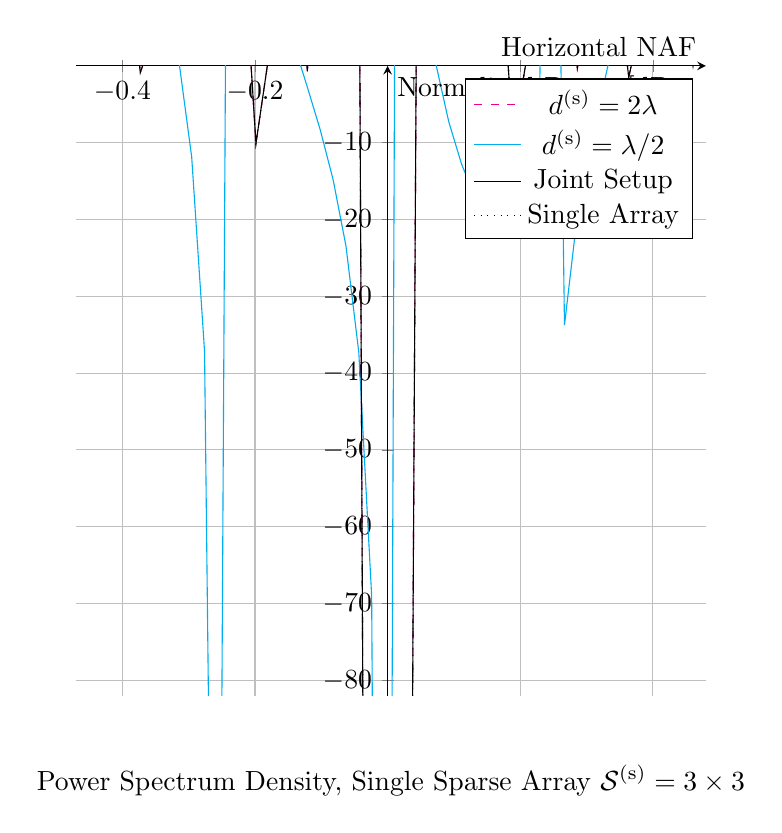
\begin{tikzpicture}
    \begin{groupplot}[group style={group size=1 by 1,vertical sep=0cm,horizontal sep=0cm},width=7cm,height=6cm,scaled ticks=false,scale only axis,xmin=-0.47,xmax=0.48,ymin=-82,ymax=0,title style={at={(0.5,-0.2)}},title={Power Spectrum Density, Single Sparse Array $\mathcal{S}^{(\mathrm{s})}=3\times3$},xlabel=Horizontal NAF,ylabel=Normalized Power [dB],legend cell align={left},legend pos=south east,legend style={font=\scriptsize},tick label style={/pgf/number format/.cd,fixed,fixed zerofill,precision=3}]
        \nextgroupplot[
            grid=major,
            axis lines=middle,
            width=8cm,height=8cm,
        ]
        \addplot[color=magenta,dashed,domain=-0.47:0.48,samples=50]{-30*cos(deg(2*pi*x))-40*cos(deg(2*pi*x)*2)-50*cos(deg(2*pi*x)*3)-60*cos(deg(2*pi*x)*4)-70*cos(deg(2*pi*x)*5)-80*cos(deg(2*pi*x)*6)-70*cos(deg(2*pi*x)*7)-60*cos(deg(2*pi*x)*8)-50*cos(deg(2*pi*x)*9)-40*cos(deg(2*pi*x)*10)-30*cos(deg(2*pi*x)*11)};
        \addlegendentry{$d^{(\mathrm{s})}=2\lambda$};
        \addplot[color=cyan,domain=-0.47:0.48,samples=50]{-30*cos(deg(2*pi*x))+cos(deg(2*pi*x)*2)-20*cos(deg(2*pi*x)*3)-10*cos(deg(2*pi*x)*4)+cos(deg(2*pi*x)*5)-10*cos(deg(2*pi*x)*6)-20*cos(deg(2*pi*x)*7)-10*cos(deg(2*pi*x)*8)+cos(deg(2*pi*x)*9)-10*cos(deg(2*pi*x)*10)-20*cos(deg(2*pi*x)*11)-10*cos(deg(2*pi*x)*12)+cos(deg(2*pi*x)*13)-10*cos(deg(2*pi*x)*14)-20*cos(deg(2*pi*x)*15)-10*cos(deg(2*pi*x)*16)+cos(deg(2*pi*x)*17)-10*cos(deg(2*pi*x)*18)-20*cos(deg(2*pi*x)*19)-10*cos(deg(2*pi*x)*20)+cos(deg(2*pi*x)*21)-10*cos(deg(2*pi*x)*22)-20*cos(deg(2*pi*x)*23)-10*cos(deg(2*pi*x)*24)+cos(deg(2*pi*x)*25)-10*cos(deg(2*pi*x)*26)-20*cos(deg(2*pi*x)*27)-10*cos(deg(2*pi*x)*28)+cos(deg(2*pi*x)*29)-10*cos(deg(2*pi*x)*30)-20*cos(deg(2*pi*x)*31)-10*cos(deg(2*pi*x)*32)+cos(deg(2*pi*x)*33)-10*cos(deg(2*pi*x)*34)-20*cos(deg(2*pi*x)*35)-10*cos(deg(2*pi*x)*36)+cos(deg(2*pi*x)*37)-10*cos(deg(2*pi*x)*38)-20*cos(deg(2*pi*x)*39)-10*cos(deg(2*pi*x)*40)+cos(deg(2*pi*x)*41)-10*cos(deg(2*pi*x)*42)-20*cos(deg(2*pi*x)*43)-10*cos(deg(2*pi*x)*44)+cos(deg(2*pi*x)*45)-10*cos(deg(2*pi*x)*46)-20*cos(deg(2*pi*x)*47)-10*cos(deg(2*pi*x)*48)};
        \addlegendentry{$d^{(\mathrm{s})}=\lambda/2$};
        \addplot[color=black,domain=-0.47:0.48,samples=50]{-30*cos(deg(2*pi*x))-40*cos(deg(2*pi*x)*2)-50*cos(deg(2*pi*x)*3)-60*cos(deg(2*pi*x)*4)-70*cos(deg(2*pi*x)*5)-80*cos(deg(2*pi*x)*6)-70*cos(deg(2*pi*x)*7)-60*cos(deg(2*pi*x)*8)-50*cos(deg(2*pi*x)*9)-40*cos(deg(2*pi*x)*10)-30*cos(deg(2*pi*x)*11)};
        \addlegendentry{Joint Setup};
        \addplot[dotted,color=black,domain=-0.47:0.48,samples=50]{-30*cos(deg(2*pi*x))-40*cos(deg(2*pi*x)*2)-50*cos(deg(2*pi*x)*3)-60*cos(deg(2*pi*x)*4)-70*cos(deg(2*pi*x)*5)-80*cos(deg(2*pi*x)*6)-70*cos(deg(2*pi*x)*7)-60*cos(deg(2*pi*x)*8)-50*cos(deg(2*pi*x)*9)-40*cos(deg(2*pi*x)*10)-30*cos(deg(2*pi*x)*11)};
        \addlegendentry{Single Array};
    \end{groupplot}
\end{tikzpicture}
\end{document}